\subsection{Measuring Rates of Change from a Table or Graph}

\begin{definition}[Slope / Rate of Change]
The slope is the ratio of vertical change to horizontal change between two points.
\end{definition}

For two points $(x_1,y_1)$ and $(x_2,y_2)$,
\[
  m=\frac{y_2-y_1}{x_2-x_1}.
\]
For a linear function $f(x)=mx+b$, the coefficient $m$ is the slope.

\subsubsection{Intervals of a Function}
When describing intervals, use interval notation such as
\[
  x\in(-\infty,a)\cup(b,\infty).
\]

\begin{remark}
Read the graph from left to right, that is, from $-\infty$ to $\infty$.
\end{remark}

\begin{example}
Here is a question by Mr. Hoken.
\begin{figure}[h!]
  \centering
  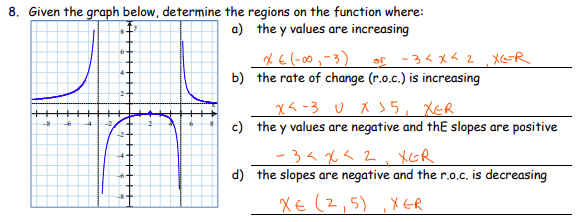
\includegraphics[width=\textwidth]{pictures/1.1.1.png}
\end{figure}

The answer for (a) is $x\in(-\infty,-3)$.

The answer for (b) is $x\in(-\infty,-3)\cup(5,\infty)$.
\end{example}

\subsubsection{Approximating the Slope of a Tangent}
Pick two points around the point of tangency with equal horizontal spacing.

Suppose points 1, 2, and 3 are on the curve, and point 2 is the tangency point.
\[
  m_1=\frac{y_2-y_1}{x_2-x_1},
  \quad
  m_2=\frac{y_3-y_2}{x_3-x_2}.
\]
An approximation of the tangent slope at point 2 is
\[
  m\approx\frac{m_1+m_2}{2}.
\]

\subsubsection{Trends: Increasing and Decreasing}
\begin{itemize}
  \item An increasing trend in $y$ corresponds to positive tangent slopes on that interval.
  \item A decreasing trend in $y$ corresponds to negative tangent slopes on that interval.
  \item "Rate of change is increasing" means slope values are increasing.
  \item "Rate of change is decreasing" means slope values are decreasing.
\end{itemize}
